\section{\ac{CPU}-\ac{GPU} Implementation}
\label{sec:CPU-GPU_Model}

The DualSPHysics code is the result of a state-of-the-art, highly optimized \ac{CPU} and \ac{GPU} implementation. The code represents the attempts to implement the best approaches for \ac{CPU} and \ac{GPU}, resulting in high accuracy, robustness and reliability. 

Preprocessing is done using GenCase \citep{Dominguez-2011b}, a robust and efficient code to manage the import of geometry files, definition of basic shapes and possible combinations, specific simulation requirements (boundary movement, different physical properties of physical entities, etc). The initial conditions represent the discretization of the defined physical entities by the intersection of these volumes with a regular Cartesian grid of spacing $Dp$, encompassing all of the domain. At every valid node a particle is created and marked according to its nature. This strategy represents the simplest but also the most robust initial condition generator available, designed for truly arbitrary scenarios, as explored in \cite{Crespo-2015}. It is possible to generate particles at given positions for further fine-tunning. Post-processing is done mostly employing Paraview \citep{Ayachit-2015}, allowing for the usage of the comprehensive filter selections and scripting capabilities for the creation of complex analysis of extensive data sets.

The simulations can be executed either on the \ac{CPU} or on the \ac{GPU} since all computations have been implemented both in C++ for \ac{CPU} and in \ac{CUDA} for the \ac{GPU}. The philosophy underlying the development of DualSPHysics is that most of the source code is common to \ac{CPU} and \ac{GPU} which makes debugging, code maintenance and the addition of new extensions straightforward. This allows the code to be run on workstations without a \ac{CUDA}-enabled \ac{GPU}, using only the \ac{CPU} implementation. On the other hand, the solver is implemented differently since code developers have considered efficient approaches for every processing unit architecture. The same programming strategy can be efficient on a \ac{CPU} but inefficient on a \ac{GPU} (or vice versa).

Algorithmically, both \ac{CPU} and \ac{GPU} simulations can be split into three main steps; i) generation of the neighbor list, ii) computation of the interactions between particles solving the system equations and iii) the update of physical quantities at the next time step using the chosen integration scheme. These three steps are repeated iteratively through the simulation.

%%%%%%%%%%%%%%%%%%%%%%%%%%%%%%%%%%%%%%%%%%%%%%%%%%%%%%%%
\subsection{\ac{CPU} Implementation}
%
The \ac{CPU} implementation is shown in Figure \ref{fig:CPU_GPU}. 
%
\begin{figure}[ht!]
	\centering
	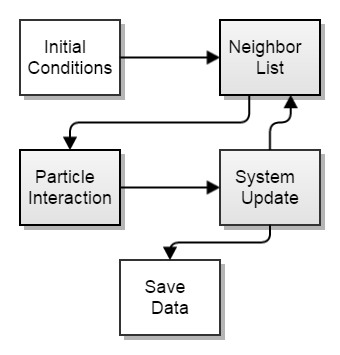
\includegraphics[width=0.35\linewidth]{Figures/4.Chapter/CPU_diagram.png}
	\caption{\small{Flowchart of \ac{CPU} implementation.}}
	\label{fig:CPU_GPU} 
\end{figure}
%

During the first step the neighbor list is generated. A cell-linked list \citep{Dominguez-2011} is generated. This process can be divided into different operations: i) domain division into square cells of side $\epsilon h$, ii) determining the cell to which each particle belongs, iii) reordering the particles according to the cells, iv) ordering all arrays with data associated to each particle and, finally, v) generating an array with the position index of the first particle of each cell. Such procedure ensures that for a particle located inside a cell, only the interactions with the particles of neighboring cells need to be considered. The number of calculations per time step is reduced from $N^2$ operations (for $N$ particles) to approximately $N\log{N}$.

Secondly, the force computation is performed so that all particle interactions are solved according to the \ac{SPH} equations. Each particle interacts with all neighboring particles located at a distance less than $\epsilon h$. Only particles inside the same cell and adjacent cells are candidates to be neighbors. Kernel symmetry, and hence kernel gradient asymmetry, avoids unnecessary repetition of particle interactions leading to a minor improvement in performance. When the force interaction of one particle with a neighbor is calculated, the force of the neighboring particle on the first one is known since they have the same magnitude but opposite direction. Thus, the number of adjacent cells to search for neighbors can be reduced if symmetry in the particle interaction is explored. Finally, the time step is computed and the quantities at step $n+1$ are calculated from the quantities that are already known at step $n$. The implementation is done using OpenMP in order to use every core of a multicore processor, and several optimizations have been implemented to ensure high performance. 

%%%%%%%%%%%%%%%%%%%%%%%%%%%%%%%%%%%%%%%%%%%%%%%%%%%%%%%
\subsection{\ac{GPU} Implementation}
%
\ac{GPU}s constitute a suitable hardware for tasks where simple calculations are carried out across large sets of data. The work presented in \cite{Crespo-2009} introduced the framework to implement \ac{SPH} codes using optimal techniques regarding performance on \ac{GPU}. That work focused on identifying suitable algorithms for efficient parallelization, since a proper and full use of all the capabilities of the \ac{GPU} architecture is not straightforward. As an initial step, the implementation focused on solving the particle interactions on a \ac{GPU} using \ac{CUDA} and the next step was the implementation of the neighbor list and the time integration in order to develop an entire \ac{GPU}-\ac{SPH}  implementation \cite{Crespo-2011}. Only output data requires transfer from \ac{GPU} to \ac{CPU}. This process, although representing a serious bottleneck due to available memory bandwidth, is rarely carried out for most applications (one out of one hundred time steps at most), representing a low percentage of the total runtime. Figure \ref{fig:GPU_flowchart} represents the single \ac{GPU} implementation. 
%
\begin{figure}[ht!]
	\centering
	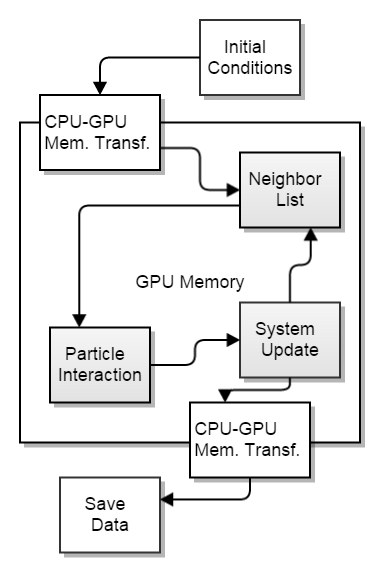
\includegraphics[width=0.35\linewidth]{Figures/4.Chapter/GPU_diagram.png}
	\caption{\small{Flowchart of \ac{GPU} implementation.}}
	\label{fig:GPU_flowchart} 
\end{figure}
%

Initially, data is allocated on \ac{CPU}, so there is a single memory transfer (from \ac{CPU} to \ac{GPU}). In all subsequent calculations, the three main steps are then performed on the \ac{GPU} device. All the sequential tasks and operations that involve a loop over all particles are performed using the parallel architecture of the \ac{GPU} cores. To save (or output) data, a new memory transfer is needed (from \ac{GPU} to \ac{CPU}). If saving data is not required all particle information remains on the \ac{GPU} memory.

The neighbor list creation follows the procedure used on a \ac{CPU}, but with important adaptations. Reordering the particles according to the cells they belong is computed using the optimized \textit{radixsort} algorithm provided by \ac{CUDA} \citep{Dominguez-2011}. Figure \ref{fig:neighbour-list} shows a simplified schematic diagram of the method used to generate an array of particle labels ordered according to cells and an array with the position index of the first and last particle in each cell. 
%
\begin{figure}[ht!]
	\centering
	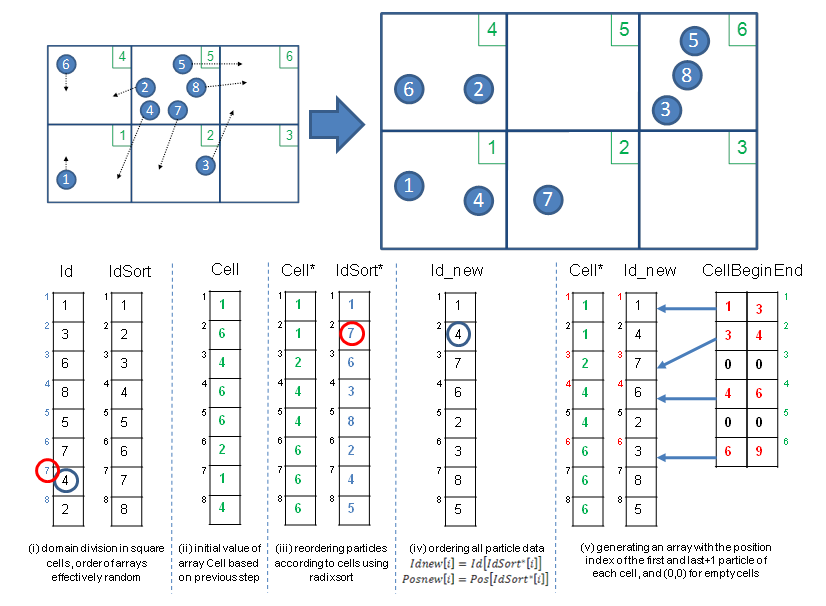
\includegraphics[scale=0.75]{Figures/4.Chapter/GPU_1_alt.png}
	\caption{\small{Example of the Neighbor list procedure \citep{Crespo-2011}}}
	\label{fig:neighbour-list} 
\end{figure}
%

Four separate arrays are used: \textit{Id, Cell, IdSort} and \textit{CellBegin} with a superscript $^*$ denoting sorted arrays. The array \textit{Id} (array of particle labels) is the starting point with particles randomly located in the domain, where the order of this array corresponds to the list of particles inherited from the previous timestep. The neighbor list is created according to the following steps:
%
\begin{enumerate}
\item Particles are stored according to the cells, so the array \textit{IdSort} is created;
\item The array \textit{Cell} is also created where an entry gives the cell to which the particle of the same index in \textit{Id} belongs, e.g. $\textit{Id}(2) = 3$ which is located in \textit{Cell 6} hence \textit{Cell(2)=6}. Cell labels are depicted in green color in Figure \ref{fig:neighbour-list}.
\item Using \textit{radixsort}, array \textit{Cell} is reordered following the order of the six cells and \textit{Cell}$^*$ (reordered \textit{Cell}) is used to reorder \textit{IdSort} according to the cells the particles belong.
\item Once \textit{IdSort}$^*$ is generated, all the arrays with particle information (\textit{Id, Position, Velocity, Density}...) are ordered giving rise to the new arrays (\textit{Id\_new, Pos\_new, Vel\_new, Dens\_new}...) considering that $\textit{Id\_new} [i] = \textit{Id} [ \textit{IdSort}^* [i] ]$. For example, $\textit{Id\_new} [2] = \textit{Id} [\textit{IdSort}^* [2] ] = \textit{Id} [7]=4$, in Figure 2 a blue circle marks the particle 4 and a red circle marks the 7th position.
\item Finally, \textit{CellBeginEnd} is created with the indexes (position in data arrays) of the first and last+1 particles of each cell. Indexes have been written in red color in Figure \ref{fig:neighbour-list}. For example the first particle of the cell number 2 is the particle 7, whose position index is 3 in all particle property arrays, so the second value of \textit{CellBeginEnd}, which corresponds to cell number 2, will be 3 and 4 (3+1). In this way, the amount of particles in the cell k will be $\textit{CellBeginEnd}[k].y-\textit{CellBeginEnd}[k].x$.
\end{enumerate}
%
Particle interactions for the computation of the forces, from equation \eqref{eq:sph_navier_momentum_I}, are a key process that must be implemented in parallel. The use of the shared memory of the \ac{GPU} was analyzed to reduce the access to the global memory. However, when the \ac{SPH} code is implemented entirely on the \ac{GPU}, this technique is not viable for current devices. For example, when the number of particles is large, the size of shared memory is not enough to allocate the properties of all the particles belonging to the same cell. 

Particle interactions were implemented on the \ac{GPU} using one execution thread per particle, to compute the force resulting from the interaction with all its neighbors. At first, this implementation seems to present some performance limitations. The workload of threads inside one block is not balanced since particles can have different numbers of neighbors. Code divergence is also a concern in this context, since the possible neighbors of a particle include both particles inside the kernel compact support ($\ve{r}_{ij}<\epsilon h$) and outside ($\ve{r}_{ij}>\epsilon h$), leading to an imbalance on the work of the threads. These limitations are made less relevant by careful usage of shared memory, function inlining and other techniques, rendering the approach the most flexible and performant option available. 

An important difference from the \ac{CPU} part of the DualSPHysics code is that the symmetry of the particle interaction cannot be applied on a \ac{GPU} implementation, since each thread is responsible for the interaction between a target particle and its neighbors. Thus, each thread must be the only one that computes the forces exerted on a given particle. The access to the global memory of the device is irregular because there is no way to organize the data to get a coalesced access for all the particles.

\subsection{Multi-\ac{GPU} \ac{MPI} Implementation}
%
The physical domain of the simulation may be divided into subdomains, distributed among different \ac{MPI} processes. Each process only needs to assign resources to manage a subset of the total amount of particles for each subdomain. Thus, the size of the simulation scales with the number of machines.

The division can be performed in any direction (X, Y or Z) according to the nature of the simulation case. The employed topology can result on two neighboring subdomains, by slicing the domain along the main direction of the problem, or in blocks, for more general cases. Each \ac{MPI} process needs to obtain, at every time step, the data of neighboring particles from the surrounding processes within the interaction distance ($\epsilon h$), in order to compute forces. This region is called the halo of the process (or subdomain). The details of the approach are further explained in \cite{Dominguez-2013b}.

Reducing time dedicated for exchanging data among \ac{MPI} processes is essential to increase the number of processes without decreasing efficiency. One method to achieve this is by overlapping the communication with the computation using asynchronous communications. One process can send (or receive) information to another while carrying out other tasks without waiting for the end of the transfer.

Figure \ref{fig:multi_gpu} shows the data exchanges that take place at each time step when using \ac{MPI}. At the beginning of each time step, during the neighbor list creation, each process looks for the particles that move from one subdomain to another and these displaced particles are sent to the corresponding process. While data of displaced particles are sent (solid arrows in Fig. \ref{fig:multi_gpu}), the neighbor list of the particles in the interior of the domain (particles not in an edge) is processed. Finally, the new particles that entered the domain are received for each process and all particles are sorted. At this stage, the computation time that is overlapped with the transfer of particles is reduced, but this is not a problem because the number of particles that change from one domain to another at each step of the simulation is typically much smaller than the number of particles in a given sub-domain.
%

\begin{figure}[ht!]
	\centering
	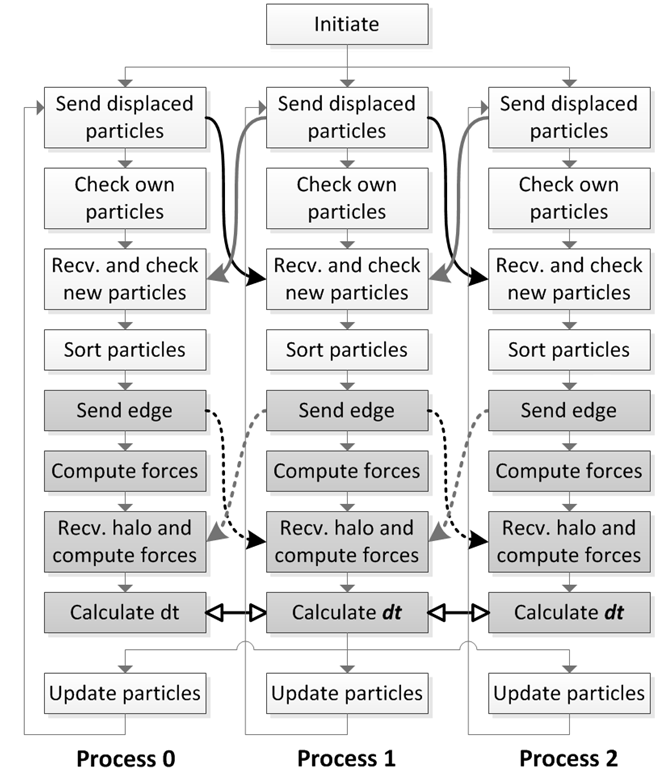
\includegraphics[scale=0.45]{Figures/4.Chapter/multi_gpu_1.png}
	\caption{\small{Example of the communications among 3 MPI processes \citep{Dominguez-2013b}}}
	\label{fig:multi_gpu} 
\end{figure}

%
During the force computation, each process sends its edges to the surrounding processes (dashed arrows in Fig. \ref{fig:multi_gpu}). While edges are being sent and the halo is received, computation of the force on the interior particles is performed. Once this is finished, the process waits for the reception of the first halo and computes forces of one edge with this halo. After that, the process waits to receive the second halo and computes the forces of the other edge. Thus the most expensive halo-edge data transfers are overlapped by calculating the forces between particles. As all particle data are allocated in the \ac{GPU} memory, data transfer is also needed between \ac{CPU} and \ac{GPU} memory. However, it should be noted that the cost is negligible since the volume of information is low and one of the advantages of the method proposed here is that the data to be transferred are stored in contiguous memory locations, accelerating the process.

Particles move through space during the simulation so the number of particles must be redistributed after some time steps to maintain a balanced work load among the processes and minimize the synchronization time. Most of the total execution time is spent on force computation, and this time depends mainly on the number of fluid particles. For an equal load per processor, the domain must be divided into subdomains with the same number of fluid particles (including particles of the halos) or with the number of particles appropriate to the computing power of the device assigned to it. Hence two different dynamic load balancing algorithms are used. The first one assigns the same number of particles to each computing device, and is suitable when the simulation is executed on machines that present the same performance. The second load balancing algorithm is used when hardware of different specifications and features are combined, such as different models of \ac{GPU}. This second approach takes into account the execution time on each device. In particular, a weighted average of the computing time per integration step over several steps is used, with a higher weight to the most recent steps. An average over many time steps is chosen because a single time step may present large fluctuations. This average time is used to distribute the number of particles so that the fastest devices can compute subdomains with more particles than the slower ones.

\subsubsection{Rigid Body \ac{MPI} Chalenges}
%
Standard \ac{SPH} is attractive for \ac{MPI} paralelization since only three sets of data from the process halos need to be exchanged: position, velocity and density, and the communication events per time step are limited. Adding rigid bodies adds a layer of complexity since relational information must be considered. The particles of the rigid bodies must be identified and treated in a separated cycle after the main interaction. Just by identifying the corresponding body, using a 2 byte array, an increase in the communicated data between processes of over $7\%$ is expected, considering only interaction.

The movement update of the rigid bodies requires the summation of quantities from all its particles, as expressed in equations \eqref{eq:rigid_linear} and \eqref{eq:rigid_angular}. As a body may be in more than one process at the same time, it is necessary to compute the partial summations on every \ac{GPU} and share those values to obtain the final configuration in all of them. In this manner, each \ac{GPU} can update its corresponding part of the rigid bodies independently. Clearly the ideal solution would be that communications were restricted between machines that shared an object, but such option forces a synchronization so that each process knew which other processes had particles from each rigid body. The best and simplest option seems to be the partial computation of the body quantities and a collective communication taking place subsequently.


